\documentclass[a4paper,article,oneside]{memoir}
\counterwithout{section}{chapter}
\usepackage{microtype}
\usepackage{longtable}
\usepackage{graphicx}
\usepackage{caption}
\newcommand{\hcp}{\textsc{hcp}}

\begin{document}

\title{Practicing Bidding on BBO}
\author{Sudhir}
\date{January 2021}
\maketitle

This document explains how to use \emph{Bridge Base Online} to
practice bidding sequences with specific reference to the \emph{COSL
  Precision} bidding system.

\section{Setting up a bidding table}

After logging in to BBO, select ``Practice'' and ``Start a Bidding Table''
from the menus. On the screen that appears next (see Figure
\ref{tablesetup}), setup your and partner's log in ids in the
North-South slots (opponents will be robots, automatically). Options
to allow kibitzers (or not) as well as whether to make the bidding
table invisible (not listed) can be set here. After the setup is
complete, press the ``Start Table'' button and this will show the table
top.

At this point, select ``Deal Source'' from the options menu as shown in
Figure \ref{dealmenu}. This opens the constraints editor that will
allow specification of the kinds of hands that are dealt. Constraints
can be set on (a) the number of high card points and (b) number of
cards in each suit.

\begin{figure}[htbp]
  \centering
  \begin{minipage}{.6\textwidth}
    \centering
    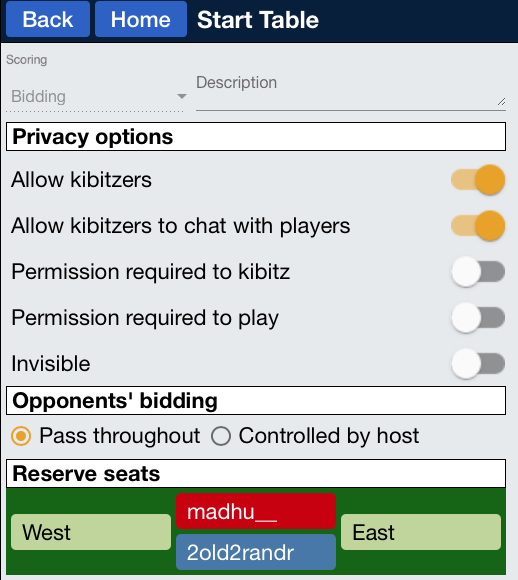
\includegraphics[width=.6\linewidth]{start-table.png}
    \captionof{figure}{Starting a bidding table}
    \label{tablesetup}
  \end{minipage}%
  \begin{minipage}{.4\textwidth}
    \centering
    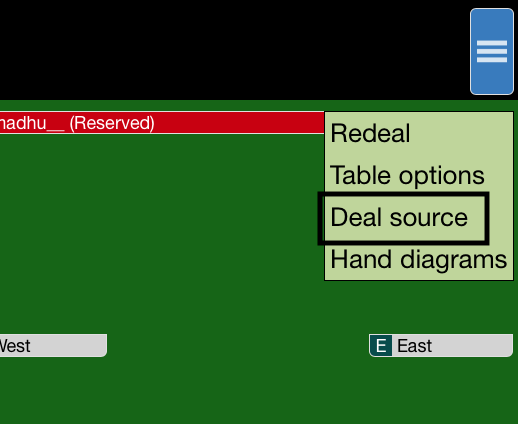
\includegraphics[width=.4\linewidth]{deal-setup.png}
    \captionof{figure}{Opening the constraints editor}
    \label{dealmenu}
  \end{minipage}
\end{figure}

In the constraints editor, several constraint sets can be defined. In
the example shown in Figures \ref{balanced} and \ref{twosuiter},
practice hands for the $1\diamondsuit$ opening are desired to be
generated. The constraints are set up to generate either 11-13\hcp\
balanced hands or 11-15\hcp\ minor two-suiters with exactly 5 clubs
and at least 5 diamonds. The option ``Randomly rotate generated deals
180 degrees'' (found in the ``Advanced'' tab) should be checked so
that opening hands are dealt to either North or South randomly
(otherwise they will be dealt only to South).

\begin{figure}[htbp]
  \centering
  \begin{minipage}{.5\textwidth}
    \centering
    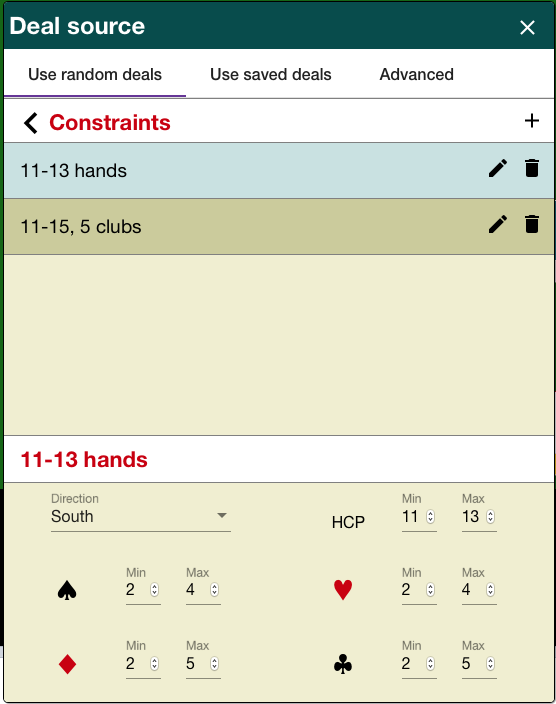
\includegraphics[width=.5\linewidth]{11-13-constraints.png}
    \captionof{figure}{11-13, balanced hands}
    \label{balanced}
  \end{minipage}%
  \begin{minipage}{.5\textwidth}
    \centering
    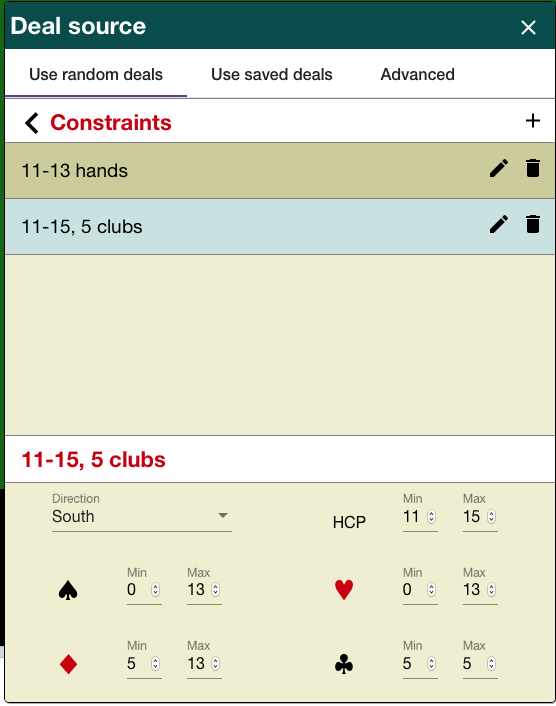
\includegraphics[width=.5\linewidth]{5-clubs-constraints.png}
    \captionof{figure}{11-15, minor two-suiters}
    \label{twosuiter}
  \end{minipage}
\end{figure}

Use the redeal menu option on the tabletop a few times to check that
the constraints are set up correctly. If all goes well, deals will be
generated to practice bidding the particular hands you are interested
in as shown in Figure \ref{sampledeal}.  Note that only one hand is
visible during bidding (partner's hand and opponents' hands are
hidden).
 
\begin{figure}[htbp]
  \centering
  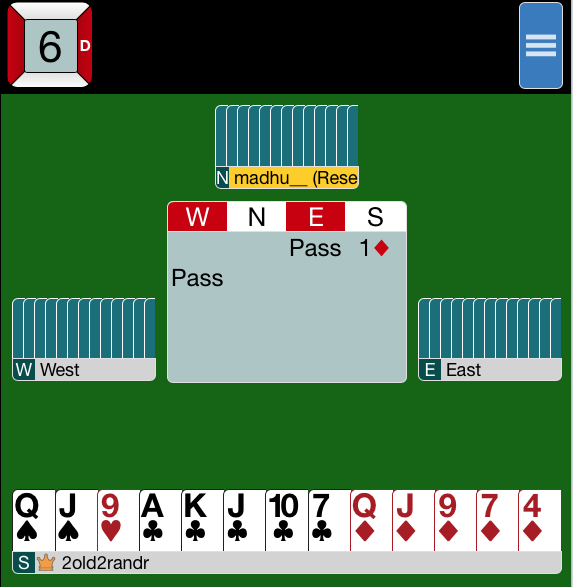
\includegraphics[width=0.8\textwidth]{sample-deal.png}
  \captionof{figure}{Sample deal}
  \label{sampledeal}
\end{figure}

\section{Constraints}

Constraints can be setup as in the table below to practice each kind
of opening hand. The next section has a study schedule that can be
used in conjunction with this table to practice bidding.

\begin{longtable}{|l|p{10cm}|}
  \hline
  $1\clubsuit$ & \hcp: 17-37. No suit constraints.

                 Omitting 16 avoids lots of 1NT openings. You may see
                 the occasional 22-23\hcp\ balanced 2NT opening coming
                 up, though. It is possible to avoid this by setting
                 up multiple constraints (17-21 any, 24-37 any, 22-23
                 unbalanced) but this is probably overkill. \\
  \hline
  $1\diamondsuit$ & \begin{tabular}{p{2.7cm}p{8cm}}
                      Balanced & 11-13\hcp,
                               $\spadesuit$ 2-4,
                               $\heartsuit$ 2-4,
                               $\diamondsuit$ 2-5,
                               $\clubsuit$ 2-5. \\
                      $\diamondsuit$ with $\heartsuit$ & 11-15\hcp,
                               $\spadesuit$ 0-1,
                               $\heartsuit$ 3-4,
                               $\diamondsuit$ 3-5,
                               $\clubsuit$ 3-5. \\
                      $\diamondsuit$ with $\spadesuit$ & 11-15\hcp,
                               $\spadesuit$ 3-4,
                               $\heartsuit$ 0-1,
                               $\diamondsuit$ 3-5,
                               $\clubsuit$ 3-5. \\
                      $\diamondsuit$ with majors & 11-15\hcp,
                               $\spadesuit$ 3-4,
                               $\heartsuit$ 3-4,
                               $\diamondsuit$ 3-5,
                               $\clubsuit$ 0-1. \\
                      $\diamondsuit$ single-suiter & 11-15\hcp,
                               $\diamondsuit$ 6-13. \\
                      Minor two-suiter & 11-15\hcp,
                               $\diamondsuit$ 5-13,
                               $\clubsuit$ 5-5. \\
                    \end{tabular} \\
  \hline
  $1\heartsuit$ & \begin{tabular}{p{2.7cm}p{6cm}}
                      Balanced & 11-13\hcp,
                               $\spadesuit$ 2-4,
                               $\heartsuit$ 5-5,
                               $\diamondsuit$ 2-4,
                               $\clubsuit$ 2-4. \\
                      Single-suited & 11-15\hcp,
                               $\heartsuit$ 6-13. \\
                      Short $\spadesuit$ & 11-15\hcp,
                               $\spadesuit$ 0-1,
                               $\heartsuit$ 5-5,
                               $\diamondsuit$ 0-5,
                               $\clubsuit$ 0-5. \\
                      Short $\diamondsuit$ & 11-15\hcp,
                               $\spadesuit$ 0-4,
                               $\heartsuit$ 5-5,
                               $\diamondsuit$ 0-1,
                               $\clubsuit$ 0-5. \\
                      Short $\clubsuit$ & 11-15\hcp,
                               $\spadesuit$ 0-4,
                               $\heartsuit$ 5-5,
                               $\diamondsuit$ 0-5,
                               $\clubsuit$ 0-1. \\
                  \end{tabular} \\
  \hline
  $1\spadesuit$ & \begin{tabular}{p{2.7cm}p{8cm}}
                      Balanced & 11-13\hcp,
                               $\spadesuit$ 5-5,
                               $\heartsuit$ 2-3,
                               $\diamondsuit$ 2-4,
                               $\clubsuit$ 2-4. \\
                      Single-suited & 11-15\hcp,
                               $\spadesuit$ 6-13. \\
                      Short $\heartsuit$ & 11-15\hcp,
                               $\spadesuit$ 5-5,
                               $\heartsuit$ 0-1,
                               $\diamondsuit$ 0-5,
                               $\clubsuit$ 0-5. \\
                      Short $\diamondsuit$ & 11-15\hcp,
                               $\spadesuit$ 5-5,
                               $\heartsuit$ 0-5,
                               $\diamondsuit$ 0-1,
                               $\clubsuit$ 0-5. \\
                      Short $\clubsuit$ & 11-15\hcp,
                               $\spadesuit$ 5-5,
                               $\heartsuit$ 0-5,
                               $\diamondsuit$ 0-5,
                               $\clubsuit$ 0-1. \\
                  \end{tabular} \\
  \hline
  1NT & 14-16\hcp, $\spadesuit$ 2-4, $\heartsuit$ 2-4,
        $\diamondsuit$ 2-5, $\clubsuit$ 2-5.

        Increase point range to 22-23 for 2NT hands. \\
  \hline
  $2\clubsuit$ & 11-15\hcp, $\clubsuit$ 6-13. \\
  \hline
  $2\diamondsuit$ & 11-15\hcp, 
                    $\spadesuit$ 3-4,
                    $\heartsuit$ 3-4,
                    $\diamondsuit$ 0-1,
                    $\clubsuit$ 4-5. \\
  \hline
\end{longtable}

For most practice sessions, no constraints need be set on the
responder's (North) hand so that the hands dealt are truly random in
terms of high-card points and distribution. However, it may be useful
to set up constraints when studying specific bidding sequences. For
example, to practice responses to one of a major over a
$1\diamondsuit$ opening, the following two constraint types could be
used on responder's hand.

\begin{longtable}{l|p{10cm}}
  \hline
  Type 1 & \hcp: 6-37,
           $\spadesuit$ 0-4,
           $\heartsuit$ 4-13,
           $\diamondsuit$ 0-13,
           $\clubsuit$ 0-13. \\
  Type 2 & \hcp: 6-37,
           $\spadesuit$ 5-5,
           $\heartsuit$ 6-13. \\
  \hline
\end{longtable}

\section{Study Plan}

The following is a 15 session plan to practice each area of the
bidding system. The schedule is based on the one in the book
``Standard Modern Precision'' by Daniel Neill.

\begin{longtable}{l|p{10cm}}
  \emph{Session} & \emph{Study Plan} \\
  \hline
  Day 1 & Practice responses to $1\diamondsuit$, the most common
          opening. Give dealer a $1\diamondsuit$ opening and responder
          6-37\hcp\ and make the correct response, but no deeper into
          the auction. Practice until the responses are easy and
          automatic. \\
  Day 2 & Still on $1\diamondsuit$, practice the special $2\clubsuit$
          and $2\diamondsuit$ responses. Give responder hands as
          below:

        \begin{tabular}{lp{8cm}}
          No 4-card major & \hcp: 13-37,
                            $\spadesuit$ 0-3,
                            $\heartsuit$ 0-3. \\
          Long $\diamondsuit$ & \hcp: 10-11, $\diamondsuit$ 6-13. \\
          Long $\clubsuit$ & \hcp: 10-11, $\clubsuit$ 6-13. \\
          Minor two-suiter, 5-card $\diamondsuit$ & \hcp: 10-11,
                                                    $\diamondsuit$ 5-13,
                                                    $\clubsuit$ 4-13. \\
          Minor two-suiter, long $\clubsuit$ & \hcp: 10-11,
                                               $\diamondsuit$ 4-4,
                                               $\clubsuit$ 5-13. \\
        \end{tabular}\\
  Day 3 & Practice $2\heartsuit$, $2\spadesuit$, $3\clubsuit$
          responses to $1\diamondsuit$. \\
  Day 4 & Practice all responses to $1\heartsuit$ and $1\spadesuit$
          openings. Remember that a limited opener can be split into
          at least three ranges for slam purposes. \\
  Day 5 & Practice all responses to a 1NT opening. Remember that the
          opener's range is 1 or 2 points stronger than standard
          Precision. \\
  Day 6 & Practice all responses to a $2\clubsuit$ opening. Be sure to
          include some practice with responder's point range set to
          14-37. \\
  Day 7 & Practice all responses to a $2\diamondsuit$ opening. For
          part of the session, set responder's point range to
          6-13. Then set responder's range to 14-37 and practice
          bidding of slam (including RKCB) or signing off in a suit
          (with or without RKCB). \\
  Day 8 & Finally, it is time to practice the strong club. Set
          responder's range to 0-7\hcp\ to practice bidding over a
          negative response. Additionally, for part of the session,
          set opener's point range to 20-37\hcp\ to develop judgement
          on when opener should force to game. \\
  Day 9 & Practice $2\heartsuit$ and $2\spadesuit$ constructive
          responses to $1\clubsuit$. Also include the positive NT
          responses in this session. \\
  Day 10 & Practice all the positive suit responses to $1\clubsuit$
           (including unusual positives). Be sure to devote some time
           to practicing the case when opener has a 4-4-4-1
           distribution with singletons in each suit.
         
           Pay special attention to reaching slams or stopping in game
           correctly. \\
  Day 11 & Practice interference by giving $2^{nd}$ seat an overcall
           in a specific suit. Give dealer a $1\diamondsuit$ opening
           and let the robots play E-W configured to generate
           overcalls. Rotate the suits in which overcalls are made and
           figure out which of responder's bids are forcing and the
           kinds of decisions opener must make when bidding
           competitively. \\
  Day 12 & Same as Day 11. \\
  Day 13 & Practice interference by $2^{nd}$ seat over a $1\clubsuit$
           opening. Again, give $2^{nd}$ seat specific suit overcalls
           with robots bidding E-W. Responder must be able to handle a
           natural overcall. Unfortunately, there is no way to make
           the robots bid 2-suited overcalls. \\
  Day 14 & A repeat of Day 8 but give $4^{th}$ seat robot some natural
           overcalls. The auction would go
           $1\clubsuit$--(Pass)--$1\diamondsuit$--(bid). \\
  Day 15 & Practice $1\clubsuit$--(Pass)--$1\heartsuit$--(bid). \\
\hline
\end{longtable}

\end{document}
